\documentclass[12pt,a4paper,oneside,openright]{book}


               %%%%%%%%%%%%%%%%%%%%%%%%%%%%%%%%%%%%%%
               % Packages			    %
               %%%%%%%%%%%%%%%%%%%%%%%%%%%%%%%%%%%%%%

\usepackage[italian]{babel}
%\usepackage[english]{babel}
\usepackage[latin1]{inputenc}
\usepackage{amsmath,amsfonts,amssymb,amsthm}
\usepackage{report}
\usepackage{fancyhdr}


               %%%%%%%%%%%%%%%%%%%%%%%%%%%%%%%%%%%%%%%%
               % First page background		      %
               %%%%%%%%%%%%%%%%%%%%%%%%%%%%%%%%%%%%%%%%
\usepackage{eso-pic}
\newcommand\BackgroundPic{
\put(0,0){
\parbox[b][\paperheight]{\paperwidth}{%
\vfill
\centering

\includegraphics[width=\paperwidth,height=\paperheight,
keepaspectratio]{figures/background.png}%
\vfill
}}}

               %%%%%%%%%%%%%%%%%%%%%%%%%%%%%%%%%%%%%%%%
               % Page size			      %
               %%%%%%%%%%%%%%%%%%%%%%%%%%%%%%%%%%%%%%%%

%\setlength{\textwidth}{12.5cm}
%\setlength{\textheight}{19cm}
%\setlength{\footskip}{3cm}

\setlength{\textwidth}{14cm}
\setlength{\textheight}{21cm}
\setlength{\footskip}{1.5cm}

\setlength{\oddsidemargin}{1cm}
\setlength{\evensidemargin}{1cm}



               %%%%%%%%%%%%%%%%%%%%%%%%%%%%%%%%%%%%%%
               % General Informations		    %
               %%%%%%%%%%%%%%%%%%%%%%%%%%%%%%%%%%%%%%


\reporttitle{Traffic Simulator}
\subject{Progetto di Reti di Telecomunicazioni L-S}
\authors{Michael Gattavecchia - \emph{0000362269}	\\
		Marco Santarelli - \emph{0000366521}	\\
		Andrea Zagnoli - \emph{0000367565}}
\courseyear{2009/10}
\faculty{II facolt\`a di Ingegneria - Cesena}
\course{Ingegneria Informatica}
\prof{ing. Walter Cerroni}
               %%%%%%%%%%%%%%%%%%%%%%%%%%%%%%%%%%%%%%
               % Contents Begin			    %
               %%%%%%%%%%%%%%%%%%%%%%%%%%%%%%%%%%%%%%

\setlength{\headheight}{15pt} %Per eliminare un Warning
\begin{document}

% Background image generation
\AddToShipoutPicture{\BackgroundPic}


%%%%%%%%%%%%%%%%%%%%%%%%%
% Introduction		%
% title, index, summary %
%%%%%%%%%%%%%%%%%%%%%%%%%
\frontmatter 
\maketitle
\pagestyle{plain} 

%%% Background image removal %%%%
\ClearShipoutPicture		%
%%%%%%%%%%%%%%%%%%%%%%%%%%%%%%%%%


\tableofcontents


%introduction
\chapter{Introduzione}
\label{ch:intro}

L'esposizione delle attivit\`a svolte \`e stata organizzata, come suggerito all'interno del documento di rifermento, in cinque macro-sezioni all'interno delle quali sono poi stati sviluppati gli argomenti specifici.
In particolare, dopo la trattazione dei generatori di numeri pseudo-casuali analizzati si passer\`a allo studio delle varie tipologie di simulazioni svolte, concludendo con l'esposizione delle attivit\`a opzionali che sono state scelte.

\subsubsection{Struttura del report}

L'implementazione del simulatore rende necessaria l'esposizione del lavoro svolto secondo un duplice punto di vista: il primo relativo alla valutazione quantitativa e qualitativa degli esiti delle simulazioni svolte, il secondo (non meno importante) relativo all'infrastruttura tecnica implementata a garanzia della validit\`a dei dati presentati. Per questo motivo, all'interno di ciascuna sezione delineata nella struttura del report sopra indicata, si \`e cercato di fornire una trattazione esaustiva di entrambi gli aspetti. In particolare, in seguito all'esposizione delle simulazioni svolte, sar\`a posta una sezione di \emph{analisi tecnica} all'interno della quale verranno esposte le particolarit\`a implementative dei componenti di volta in volta coinvolti.
\\

La piattaforma di riferimento per lo sviluppo del simulatore \`e \emph{Java}, attraverso la quale sono stati sviluppati sia il simulatore in s\'e, sia la parte relativa alla costruzine dei grafici relativi alle simulazioni svolte.

\newpage
\subsubsection{Gruppo di lavoro}

Il gruppo di lavoro \`e costituito da:
\begin{itemize}
\item Michael Gattavecchia - \emph{0000362269}	
\item Marco Santarelli - \emph{0000366521}	
\item Andrea Zagnoli - \emph{0000367565}
\end{itemize}


%%%%%%%%%%%%%%%%%%%%%%%%%
% Document's body	%
%%%%%%%%%%%%%%%%%%%%%%%%%
\mainmatter

% pagestyle
\pagestyle{fancy} \fancyhead[LE,RO]{\bfseries\thepage}


% chapters
\chapter{Generazione di numeri pseudo-casuali}
\label{ch:rnd}

Alla base di una qualsivolglia simulazione risiede la centralit\`a del ruolo rivestito dalla riproduzione dell'aleatoriet\`a riscontrabile all'interno dei sistemi reali. Per questo motivo \`e fondamentale valutare e conoscere le entit\`a alle quali si fa riferimento per la generazione di numeri casuali, il cui comportamento incider\`a in maniera rilevante sulla qualit\`a delle simulazioni.

Per la generazione di numeri pseudo-casuali sono stati considerati, in fase di analisi, quattro metodologie alternative, le cui caratteristiche sono riportate all'interno dell'apposita scheda presente nell'interfaccia grafica del simulatore:
\begin{itemize}
\item {\tt java.util.Random}\\
	generatore predefinito dell'environment Java per la generazione di numeri pseudo-casuali.
\item {\tt ran0}\\
	generatore lineare congruenziale di tipo \emph{ran0}, implementato ex-novo.
\item {\tt SecureRandom}\\
	generatore presente all'interno del package {\tt java.security} in grado di generare sequenze pseudo-casuali crittograficamente robuste.
\item {\tt MersenneTwister}\\
	generatore implementato all'interno del progetto Apache che realizza l'algoritmo Matsumoto-Nishimura.
\end{itemize}


\section{Generatori lineari congruenziali}

I generatori lineari congruenziali rappresentano una tra le pi\`u conosciute e sperimentate alternative per la generazione di numeri pseudo-casuali. 

Il meccanismo di generazione \`e definito, ricorsivamente, come:

$$
Z_{i}=(a \cdot Z_{i-1}+c)\mod m
$$

dove:\\
$Z_{i}$ rappresenta l'i-esima istanza generata\\
$m \thickspace(0<m)$		, il modulo\\
$a \thickspace(0<a<m)$		, il ``moltiplicatore''\\
$c \thickspace(0\le c<m)$	, l'incremento\\
$Z_{0}$ il seme della sequenza (seed)\\

Il periodo di un generatore lineare congruenziale \`e al pi\`u pari a $m$\footnote{in questo caso il periodo del generatore \`e detto ``pieno''.}, a patto di rispettare alcuni vincoli:
\begin{itemize}
\item[-] $c$ ed $m$ siano coprimi tra loro
\item[-] $(a-1)$ sia divisibile per tutti i fattori primi di m
\item[-] $(a-1)$ sia multiplo di 4, qualora anche $m$ lo sia
\end{itemize}

Le modalit\`a secondo le quali questo tipo di generatori sono definiti fanno s\`i che essi siano particolarmente apprezzati per la loro leggerezza, vista la necessit\`a di memorizzare le sole variabili di stato per un corretto funzionamento e la semplicit\`a dei calcoli necessari per la generazione. Moltiplicazioni tra interi ed il calcolo del modulo sono infatti operazioni che un moderno microprocessore pu\`o realizzare in maniera molto performante.
Tuttavia esiste correlazione tra i valori generati successivamente, che determina l'impossibilit\`a di utilizzare questo tipo di generatori in ambienti in cui tale correlazione rappresenti un fattore di rischio, come ad esempio in ambito crittografico.

\subsection{Classe {\tt Random}}
\label{sec:rndjava}
La classe {\tt Random}, presente all'interno del package {\tt java.util}, rappresenta lo standard per la generazione di valori pseudo-casuali all'interno dell'environment Java.


\begin{table}[!h]
	\begin{center}
	\begin{tabular}{c|c}
	parametro & valore\\
	\hline
	$m$ & $2^{48}$  \\
	$a$ & $25214903917$  \\
	$c$ & $11$  \\
	\end{tabular}
	\end{center}
	\caption{Parametri del LCG implementato in {\tt java.util.Random}}
	\label{tab:rndjava}
\end{table}

Si tratta di un LCG caratterizzato dai parametri mostrati in tab.\ref{tab:rndjava}
e dotato quindi di un periodo pari a  $2^{48} \thickspace (281,474,976,710,656)$.
Un'istanza della classe {\tt Random} permette di ``prelevare'' valori pseudo-casuali di diverso tipo a seconda delle necessit\`a, mediante l'invocazione parametrizzata del metodo protetto {\tt next()}.

Il seme della sequenza pseudo-casuale, formato da 48 bit, pu\`o essere specificato in modo esplicito all'atto della costruzione ({\tt Random(long seed)}), o acquisito tramite l'invocazione interna del metodo {\tt System.currentTimeMillis()} nel caso in cui si ricorra al costruttore standard.

\subsection{Generatore {\tt ran0}}

Il generatore realizzato ex-novo per il simulatore \`e di tipo lineare congruenziale (\emph{ran0}). Come possibile osservare in tabella \ref{tab:rndcustom}, il parametro $c$ \`e stato posto uguale a $0$: questo caratterizza il generatore come di tipo ``Park-Miller'' (moltiplicativo).

Analogamente a quanto visto nel caso del LCG standard di Java, il generatore pu\`o o meno essere instanziato unitamente ad un seed di partenza. In caso tale parametro venga omesso si ricorrer\`a nuovamente alla chiamata 
{\tt System.currentTimeMillis()} per l'ottenimento di un valore arbitrario da impostare come seed iniziale.

\begin{table}[!h]
	\begin{center}
	\begin{tabular}{c|c}
	parametro & valore\\
	\hline
	$m$ & $2147483647$  \\
	$a$ & $16807$  \\
	$c$ & $0$  \\
	\end{tabular}
	\end{center}
	\caption{Parametri del LCG implementato ex-novo ({\tt RandomProvider})}
	\label{tab:rndcustom}
\end{table}

\subsection{SecureRandom}

La classe {\tt SecureRandom} presente all'interno del package {\tt java.security} estende la classe {\tt Random} discussa in precedenza, e permette la generazione robusta dal punto di vista crittografico di numeri pseudo-casuali attraverso l'agoritmo\footnote{e.g. {\tt ``SHA1PRNG''} che segue le specifiche dello standard IEEE P1363} e l'eventuale provider specificati nella chiamata di instanziamento.

Il seed verr\`a poi automaticamente generato attraverso l'invocazione automatica del metodo {\tt setSeed()}.

\subsection{MersenneTwister}

La classe {\tt MersenneTwister}, sviluppata dal progetto \emph{Apache} e disponibile all'interno del package {\tt commons.math.random.MersenneTwister}, implementa l'algoritmo ideato da Makoto Matsumoto e Takuji Nishimura nel 1996/97. 

Questo generatore \`e caratterizzato da un periodo parcolarmente lungo (pari a $2^{19937}-1$), da una equidistribuzione a 623 dimensioni e da una accuratezza massima pari a 32 bit.

L'algoritmo \`e basato sulla seguente ricorsione lineare:

$$x_{k+n}:=x_{k+m} \oplus (x_{k}^{u}|x_{k+1}^{l})A, (k=0,1,...)$$

per il cui approfondimento si rimanda alla bibliografia \cite{matsumoto}.

\subsection{Analisi tecnica: classe {\tt RandomProvider}}

All'interno della classe {\tt RandomProvider}, oltre al generatore creato ex-novo, vengono gestite tutte le tipologie di generatori disponibili, elencate all'interno dell'{\tt enum Provider}. In particolare all'interno della chiamata per l'instanziamento \`e possibile specificare la tipologia di generatore che si intende utilizzare, permettendo una fruizione del servizio disaccoppiata dalla specifica implementazione scelta.

\section{Analisi del generatore}

Il generatore che si \`e scelto di utilizzare come default per il simulatore \`e quello fornito dalla classe {\tt Random} di Java. Tale scelta \`e stata dettata dalla estrema efficienza computazionale di tale generatore e dalla trascurabile rievanza degli effetti della correlazione per l'applicazione di interesse.

\subsection{Distribuzione uniforme in [0,1]}

Per la valutazione dell'uniformit\`a della distribuzione dei valori generati si \`e deciso di realizzare uno scatter plot. Per la realizzazione di questo grafico \`e necessaria la generazione di $N$ coppie di numeri pseudo-casuali, i quali devono essere generati in modo consecutivo, senza variare il seme dell'algoritmo di generazione. Le coppie generate sono quindi utilizzate come le coordinate $X$ e $Y$ dei punti da mostrare nel grafico. Nel caso pi\`u generale \`e possibile specificare un numero variabile di generazioni che devono essere effettuate per ogni coppia tra la coordinata dell'ascissa e dell'ordinata: nel nostro caso si \`e scelto di usare la generazione immediatamente successiva a quella dell'ascissa. Questo grafico permette di individuare correlazioni evidenti tra i valori o problemi dovuti a parametri critici dell'algoritmo, che si presentano come disposizioni ordinate dei punti del grafico.   In figura \ref{fig:random} si mostra la distribuzione dei valori generati da un'istanza della classe Random: \`e possibile apprezzare il buon livello di dispersione e la discreta uniformit\`a dei punti nella copertura dello spazio.
La sezione del simulatore dedicata all'analisi di generatori di numeri random permette di creare dinamicamente scatter plot per ciascuna delle 4 tipologie di generatori discussi in precedenza.



\begin{figure}[!h]{
	\begin{center}
	   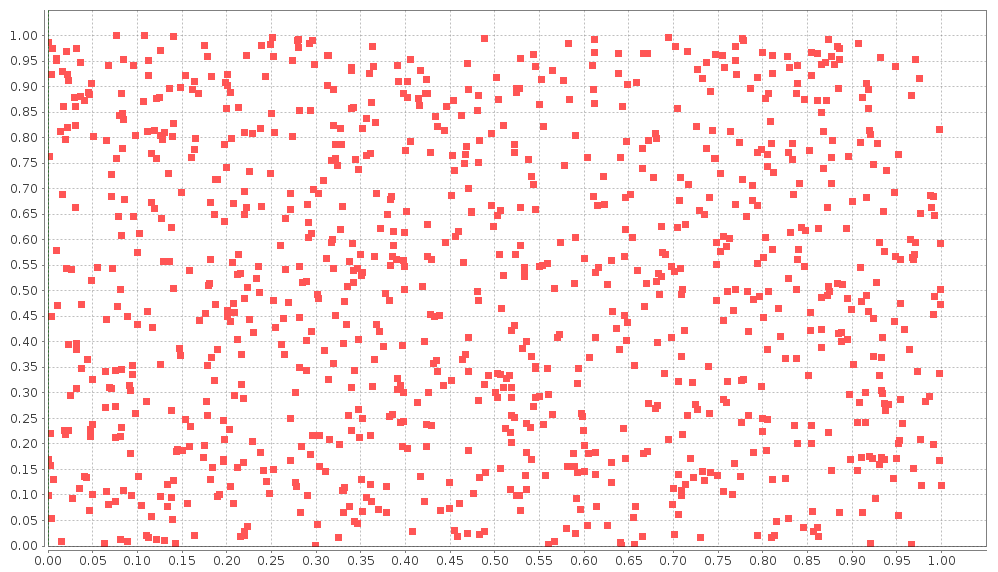
\includegraphics[width=0.95\textwidth]{figures/random.png}
	\end{center}}
	\caption{Distribuzione dei valori generati da {\tt util.Random}}
	\label{fig:random}
\end{figure}


\subsection{Stima del valore medio}

Al fine di permettere un'agevole valutazione visiva del valor medio delle sequenze di numeri pseudo-casuali prodotte si \`e ricorsi ad una serie di generazioni con campioni di dimensione crescente.

\begin{figure}[!h]{
	\begin{center}
	   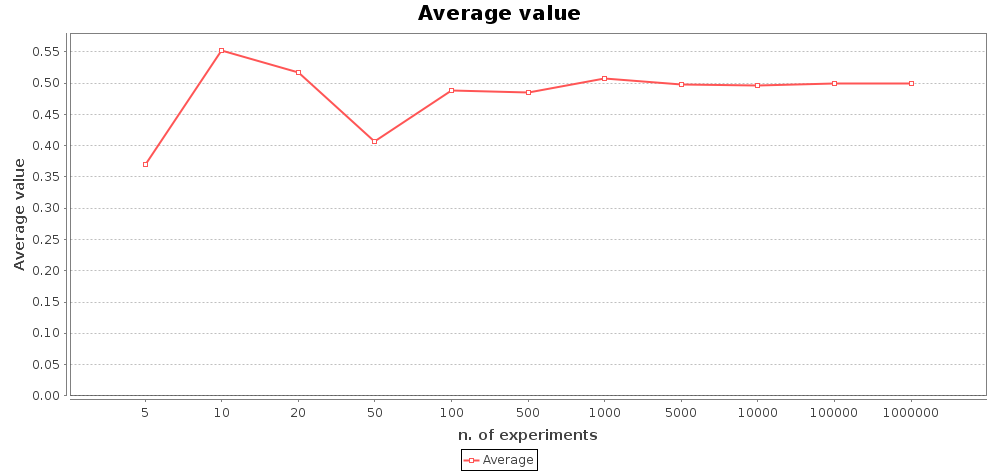
\includegraphics[width=0.95	\textwidth]{figures/average.png}
	\end{center}}
	\caption{Media dei campioni in funzione della numerosit\`a}
	\label{fig:avg}
\end{figure}

In figura \ref{fig:avg} \`e possibile osservare come, all'aumentare della dimensione dei campioni, si abbia una convergenza al valore teorico di $0.5$.
In particolare, gi\`a a partire da qualche migliaio di esperimenti, si pu\`o osservare un'importante grado di aderenza al valore teorico. 

L'andamento della media campionaria presenta sempre ad ogni ripetizione dell'esperienza la stessa tendenza a convergere al valore teorico atteso, con oscillazioni rilevanti presenti esclusivamente in concomitanza ai campioni di piccole dimensioni, come era lecito attendersi.

Anche per l'analisi del valor medio dei numeri pseudo-casuali generati \`e possibile selezionare le varie tipologie di generatori messe a disposizione, ottenendo di volta in volta il relativo grafico.

\subsection{Intervallo di confidenza}

Per la valutazione degli intervalli di confidenza sono state effettuati esperimenti sia al variare del livello di confidenza, sia al variare del numero di campioni. 
Come era lecito aspettarsi, l'intervallo di confidenza mostra un andamento decrescente all'aumentare del numero di campioni presi in considerazione, mentre ha un'andamento crescente all'aumentare del livello di confidenza richiesto.
I grafici ci hanno permesso inoltre di confrontare quantitativamente i valori calcolati dalle funzionalit\`a da noi realizzate con i valori teorici, confermandoci la loro corretta implementazione

\begin{figure}[!h]{
	\begin{center}
	   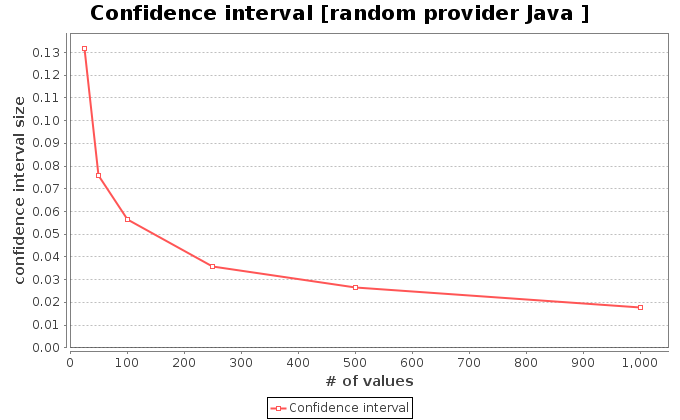
\includegraphics[width=\textwidth]{figures/IDC_1.png}
	\end{center}}
	\caption{Intervallo di confidenza in funzione del numero di campioni}
	\label{fig:idc1}
\end{figure}

In fig.\ref{fig:idc1} e \ref{fig:idc2} \`e possibile osservare l'andamento dell'IDC in funzione del numero di esperimenti svolti e del livello di confidenza, rispettivamente.

\begin{figure}[!h]{
	\begin{center}
	   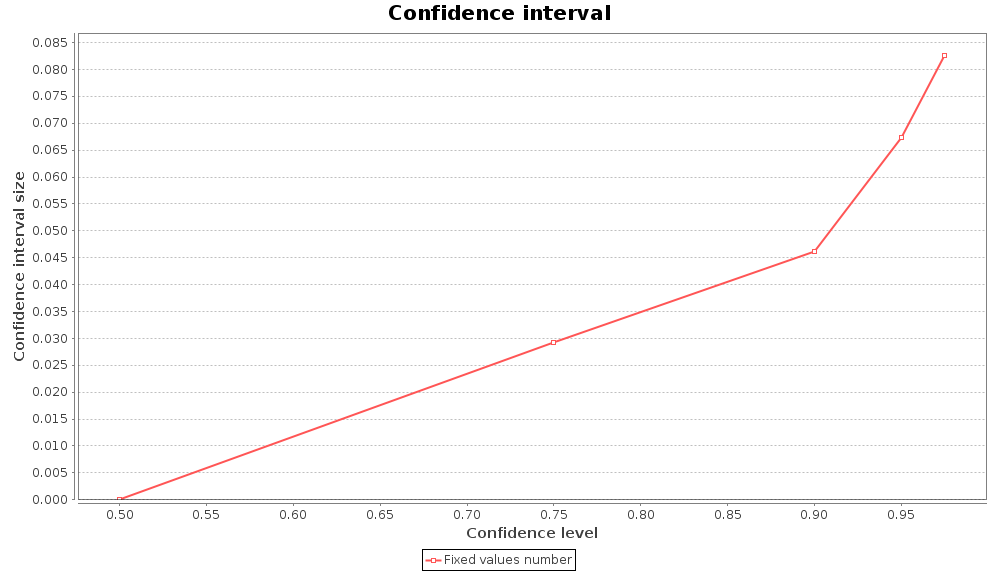
\includegraphics[width=\textwidth]{figures/IDC_2.png}
	\end{center}}
	\caption{Intervallo di confidenza in funzione del livello di confidenza}
	\label{fig:idc2}
\end{figure}

\subsection{Analisi tecnica}

L'esecuzione effettiva delle due possibili tipologie di simulazione per il calcolo dell'intervallo di confidenza (in funzione del numero di run o del livello di confidenza) \`e opera, rispettivamente,  dei metodi:
\begin{itemize}
\item {\tt testConfidenceIntervalWithVariableConfidence(...)} 
\item {\tt testConfidenceIntervalWithVariableRuns(...)}
\end{itemize} 

della classe {\tt SimulationRunners}. All'interno di quest'ultima sono stati infatti raccolti, al fine di ottenere una struttura topologicamente ben organizzata,  i metodi corrispondenti alle varie tipologie di esperimenti messi a disposizione dal simulatore implementato.

All'utente viene data la possibilit\`a di scegliere un generatore di numeri pseudo-casuali tra i quattro esposti al capitolo \ref{ch:rnd}, e di specificare la tipologia di simulazione ed il relativo parametro di riferimento. 

Una volta terminata la parte computazionale, attraverso un apposito metodo della classe {\tt gui.GraphUtils}, viene generato e visualizzato un grafico riportante gli esiti della simulazione.

La classe {\tt GraphUtils} verr\`a in seguito utilizzata per la creazione della totalit\`a dei grafici generati a seguito delle simulazioni, vista la volont\`a di mantenere una strutturazione ben organizzata di classi e package all'interno del progetto.

\subsection{Realizzazione dei grafici}
Per la realizzazione dei grafici relativi alle simulazioni si \`e ricorsi all'utilizzo del tool gratuito \emph{JFreeChart}\footnote{http://www.jfree.org/jfreechart/}, che permette la realizzazione di grafici all'interno dell'invironment Java, oltre a permettere l'esportazione degli stessi in diversi formati di immagine (png).
JFreeChart mette a disposizione numerose tipologie di grafici e diagrammi, consentendo una gamma di personalizzazioni pressoch\'e illimitata.
Si \`e deciso di appoggiarsi a questa libreria poich\'e, implementando il simulatore in Java, si ha l'indubbio vantaggio di poter mostrare i grafici direttamente da codice, senza bisogno di utilizzare tool esterni e senza dover estrarre ed esportare i dati dal simulatore. Inoltre, il framework che la libreria mette a disposizione consente di navigare, ridimensionare, zoomare ed editare i chart tramite interfaccia grafica, consentendoci di ottimizzare la presentazione dei dati in maniera pi\`u rapida.

%\begin{figure}{
%	\begin{center}
%	   \includegraphics[width=\textwidth]{figures/esempi.png}
%	\end{center}}
%	\caption{Tipologie ricorrenti di artefatti: boundary artifacts (B), resource artifacts (R), coordination %%artifacts (C).}
%	\label{fig:esempi}
%\end{figure}

%\begin{table}
%	\begin{center}
%	\begin{tabular}{c|c}
%	Title & $ values $\\
%	\hline
%	10 &  0.5741\\	
%	\end{tabular}
%	\end{center}
%	\caption{Valori medi relativi ai valori generati}.
%	\label{tab:media}e
%\end{table}

\chapter{Generazione di traffico con diversa variabilit\`a}

\section{Distribuzioni di traffico considerate}

Le distribuzioni secondo le quali il traffico si presenta all'ingresso del sistema influenzano in modo marcato le dinamiche che a regime vengono a determinarsi all'interno dello stesso. Per questo motivo \`e di grande importanza osservare la risposta specifica del sistema ad input differenziati, al fine di valutarne le caratteristiche e di meglio comprendere le specifiche peculiarit\`a delle varie distribuzioni in analisi.

Le tipologie di distribuzione prese in considerazione sono, come da specifica:
\begin{itemize}
\item Deterministica 
\item Poissoniana (Exponential)
\item Switched Poisson Process (SPP) 
\item Pareto
\end{itemize}

Il simulatore permette, in funzione del tipo di distribuzione selezionata e dei parametri imposti, di valutare valore medio, varianza ed indice di dispersione relativi al traffico generato.

\begin{figure}[!h]{
	\begin{center}
	   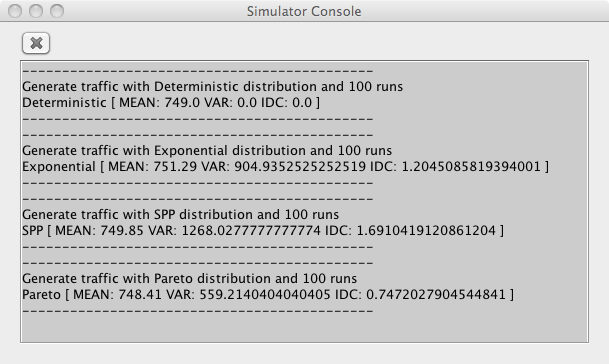
\includegraphics[width=\textwidth]{figures/simconsole.png}
	\end{center}}
	\caption{Esito della simulazione di varie tipologie di traffico (console)}
	\label{fig:console}
\end{figure}


Al termine della computazione, i risultati numerici vengono riportati sulla console appositamente realizzata (fig. \ref{fig:console}).


\subsection{Analisi tecnica}

L'esecuzione della simulazione avviene, analogamente a quanto visto nel capitolo precedente, facendo ricorso alla classe {\tt SimulationRunners}. L'organizzazione gerarchica delle distribuzioni, ottenuta mediante varie specializzazioni della classe {\tt Distribution} rende possibile una gestione trasparente rispetto alla scelta effettuata dall'utente.

Per la gestione della console di sistema, all'interno della quale vengono presentati i risultati delle simulazioni, si \`e ricorsi alla libreria LOG4J\footnote{LOG4J - http://logging.apache.org/log4j/1.2/}
In particolare si \`e realizzata una console su finestra indipendente la cui visualizzazione pu\`o essere (dis)abilitata dall'utente, senza che i dati in essa contenuti vadano persi.

\begin{figure}[!h]{
	\begin{center}
	   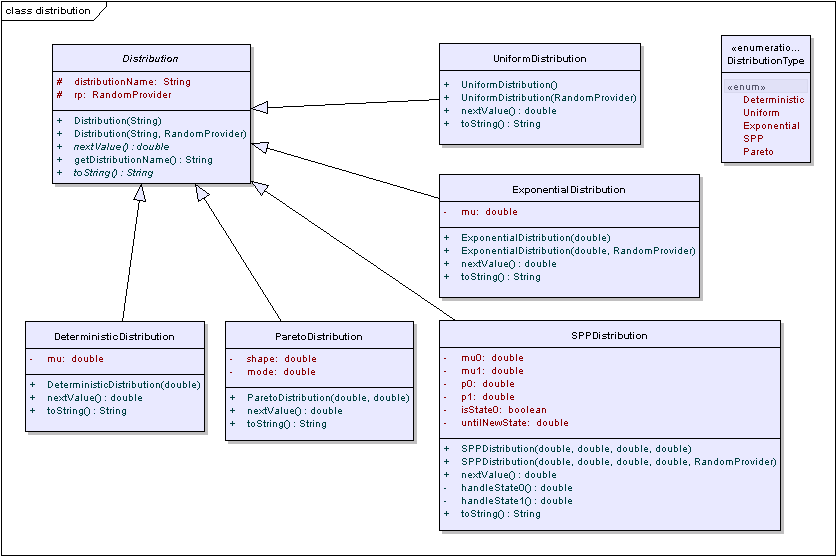
\includegraphics[width=\textwidth]{figures/distributionclass.png}
	\end{center}}
	\caption{Struttura del package {\tt simulator.distribution}}
	\label{fig:distuml}
\end{figure}

La generazione di valori da parte delle classi che implementano la classe astratta {\tt Distribution} (si veda lo schema in fig \ref{fig:distuml}) avviene attraverso il metodo {\tt nextDouble()}, in particolare ogni estensione della classe implementa una spefica funzione in base al tipo di distribuzione rappresentato.

Infine, \`e interessante notare come attraverso il ricorso alla classe {\tt Executor- Service} l'onere computazionale sia stato scisso dalla gestione dell'interfaccia grafica, permettendo cos\`i un'esperienza d'utilizzo esente da blocchi dovuti alla computazione.

%ACHTUNG: su ExecutorService (sopra) si "forza" un acapo manuale, brutto brutto brutto!

%\subsubsection{Nota}
%Per la simulazione di traffico con diversa variabilit\`a trattata in questo capitolo, e per le successive, si \`e fatto affidamento sulla classe {\tt Random} descritta in sezione \ref{sec:rndjava}, date l'ottima efficienza computazionale dello stesso e la scarsa incisivit\`a dei difetti comuni ai generatori lineari congruenziali in genere per l'applicazione in oggetto.

\chapter{Simulazione di una coda $M/G/1$}
\label{ch:mg1}

\section{Sistema a coda $M/G/1$}

Il sistema considerato in questo capitolo \`e di tipo a singolo servitore, con arrivi di tipo poissoniano, tempi di servizio variabilmente distribuiti e media $\mu$ definiti dall'utente in fase di inizializzazione.

\begin{figure}[!h]{
	\begin{center}
	   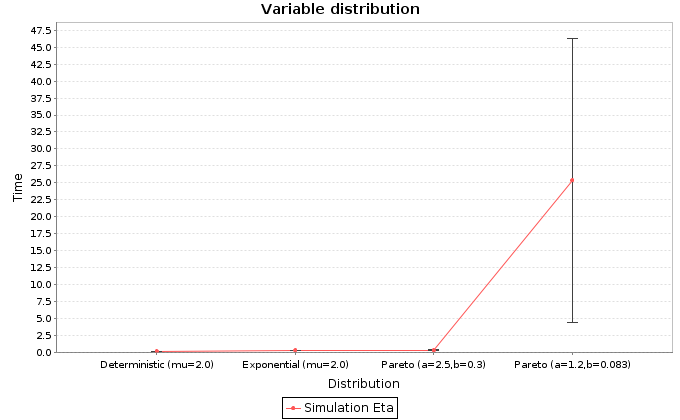
\includegraphics[width=\textwidth]{figures/mg1dists.png}
	\end{center}}
	\caption{Tempi medi di attesa al variare del tipo di distribuzione $\rho=0.4$, $\mu=2.0$, $N=100$}
	\label{fig:mg1dists}
\end{figure}

\begin{figure}[!h]{
	\begin{center}
	   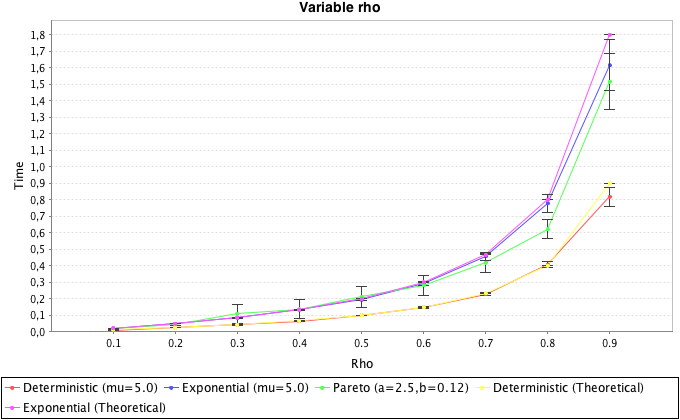
\includegraphics[width=\textwidth]{figures/cfrdists.png}
	\end{center}}
	\caption{Tempi medi di attesa al variare di $\rho$ per i vari tipi di distribuzione}
	\label{fig:cfrdists}
\end{figure}

La simulazione di una coda di tipo $M/G/1$ pu\`o essere effettuata, come da specifica richiesta, in funzione delle varie tipologie di distribuzione o in funzione della variazione supervisionata di $\rho$ nell'intervallo $(0,1)$.

\begin{figure}[!h]{
	\begin{center}
	   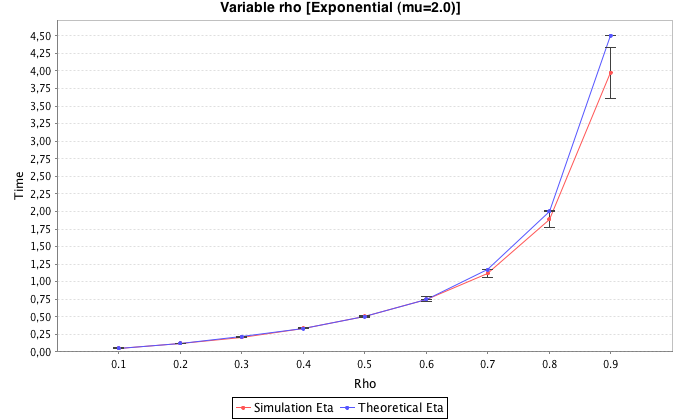
\includegraphics[width=\textwidth]{figures/mg1expmu2.png}
	\end{center}}
	\caption{Tempi medi di attesa al variare di $\rho$ con distribuzione Poissoniana dei tempi di servizio}
	\label{fig:mg1expmu2}
\end{figure}

\begin{figure}[!h]{
	\begin{center}
	   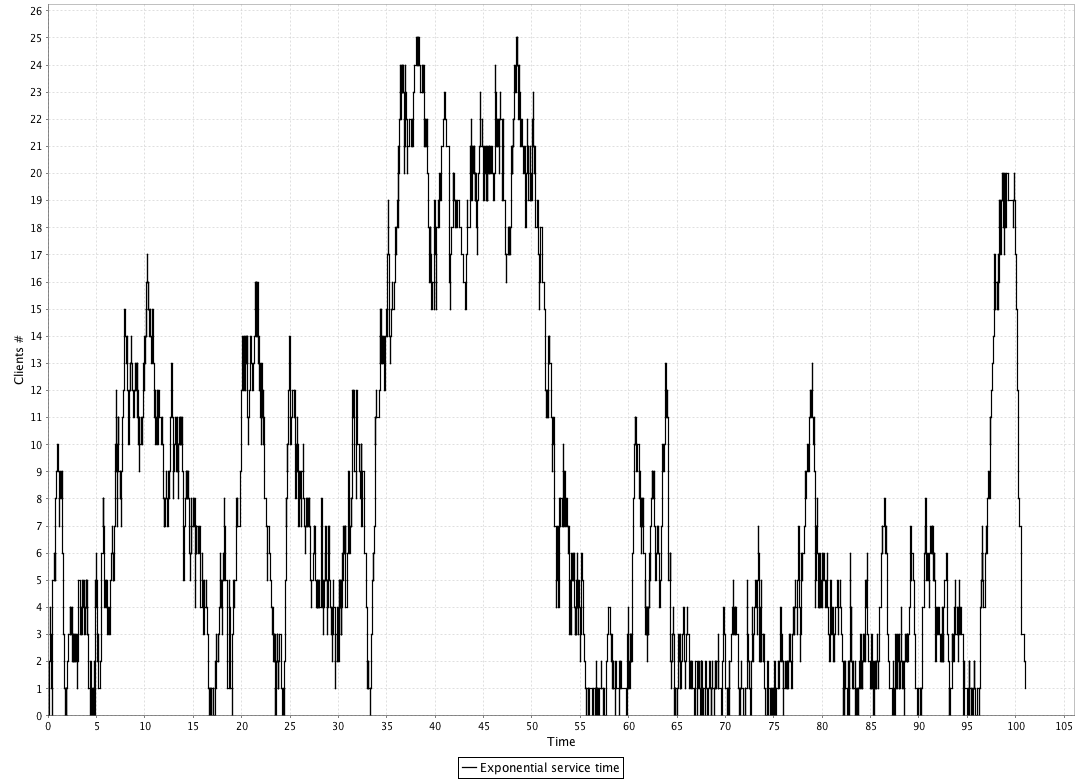
\includegraphics[width=\textwidth]{figures/kt.png}
	\end{center}}
	\caption{Numero di utenti nel sistema $k(t)$ in funzione del tempo, durante una simulazione}
	\label{fig:kt}
\end{figure}

La simulazione in funzione della tipologia di distribuzione permette di apprezzare, analogamente a quanto visto in fase di analisi teorica, come la distribuzione di Pareto configurata con parametro $1<\alpha\le2$ presenti un'estrema variabilit\`a, soprattutto se postaa confronto con traffico di tipo Poissoniano o deterministico (figura \ref{fig:mg1dists}).

La simulazione in funzione della variazione di $\rho$\footnote{la simulazione \`e stata realizzata facendo variare $\rho$ nell'intervallo $[0.1, 0.9]$ con passo di incremento pari a $0.1$} evidenzia la tendenza a divergere del tempo medio di attesa nel sistema $\eta$ al crescere dell'occupazione dell'unico servitore presente. In figura \ref{fig:mg1expmu2} \`e possibile notare come la caratterizzazione qualitativa e quantitativa dei dati ricalchi in maniera molto fedele l'andamento della curva teorica relativa ai sistemi $M/G/1$.

All'interno della scheda dedicata alla simulazione della coda $M/G/1$ \`e possibile notare l'opzione relativa alla stima della probabilit\`a di stato della coda, tale opzione \`e parte delle simulazioni a scelta implementate e verr\`a meglio esposta al capitolo \ref{ch:optional}.


\subsection{Analisi tecnica}

La struttura del simulatore \`e stata definita in aderenza alle specifiche fornite all'interno delle slide a supporto del corso \cite{cerroni01}. 
Al fine aggiuntivo di conferire al sistema una migliore strutturazione dal punto di vista dell'ingegneria del software si \`e deciso di implementare una classe astratta {\tt Simulator}, svincolata dalla specifica politica di gestione delle code utilizzata. 

Tale polica viene infatti gestita specificamente all'interno di due specializzazioni della suddetta classe, tali {\tt FCFSSimulator} e {\tt SJNSimulator}, che nell'ordine realizzano un simulatore in cui la politica di servizio \`e \emph{``first-come/first-served''} e \emph{``shortest-job next''}.

La gestione della simulazione viene, in fase preliminare, gestita all'interno del pannello dell'interfaccia grafica dedicato. Dopo l'analisi della correttezza dell'input per\`o, al fine di garantire il massimo disaccoppiamento tra elborazione dati e interazione con l'utente, viene generato un nuovo thread che tramite l'utilizzo di metodi dedicati della classe {\tt SimulationRunners} permette lo svolgimento effettivo della simulazione. Al termine di quest'ultima verranno quindi generati eventuali grafici e/o output in console.

\begin{figure}[!h]{
	\begin{center}
	   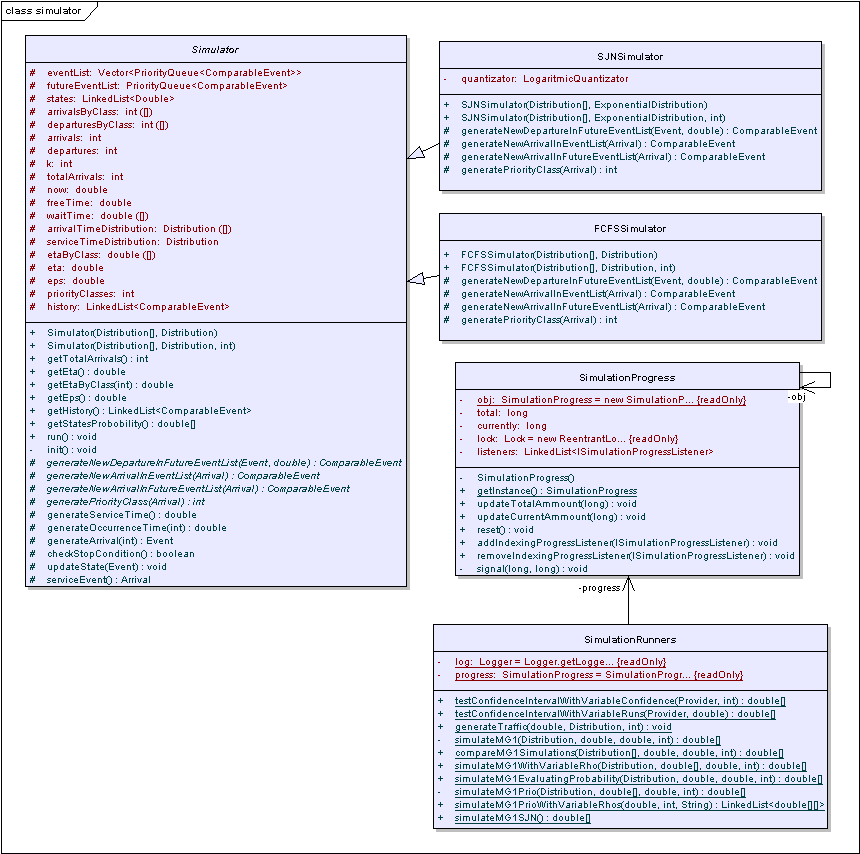
\includegraphics[width=\textwidth]{figures/simulatorclass.png}
	\end{center}}
	\caption{Struttura del package {\tt simulator}}
	\label{fig:simulatorclass}
\end{figure}

Un'ulteriore accorgimento messo in atto per evitare l'andarsi a delineare di situazione di forte concorrenza in fase di esecuzione\footnote{vista anche la grande richiesta computazionale in fase di simulazione, determinata da una sostanziale prevalenza di cicli cpu-burst.} \`e il ricorso alla classe {\tt ExecutorService}. In particolare, l'esecuzione delle simulazioni viene in tutte le sue forme demandata ad un istanza della classe {\tt ExecutorService} instanziata attraverso l'invocazione del costruttore {\tt newSingleThreadExecutor()} della classe {\tt Executor}, che di fatto permette l'utilizzo controllato di un singolo thread per le operazioni a maggior carico computazionale.

In figura \ref{fig:simulatorclass} \`e possibile osservare la strutturazione definita per entit\`a dedicate alla simulazione.


\chapter{Simulazione di una coda $M/G/1//Prio$}

\section{Sistema a coda $M/G/1//Prio$}


Per la simulazione di un sistema a coda con classi di priorit\`a assegnata agli utenti \`e possibile, attreverso l'opportuna scheda, selezionare le varie configurazioni per la caratterizzazione delle classi.

Tali configurazioni comprendono, in aderenza alle specifiche fornite, due o tre classi alle quali sono associate differenti priorit\`a. Per la specificit\`a delle stesse si rimanda alla tabella \ref{tab:mg1prioclasses}.

\begin{table}[!h]
	\begin{center}
	\begin{tabular}{|ccl|}
	\hline
	ID  & n. classi & caratteristiche\\
	\hline
	2 & 2 & $\rho_{1}=x\rho$  \\
	& & $\rho_{2}=(1-x)\rho$ \\
	\hline
	3a & 3 & $\rho_{1}={x\over2}\rho$  \\
	& & $\rho_{2}={x\over2}\rho$  \\
	& & $\rho_{3}=(1-x)\rho$  \\
	\hline
	3b & 3 & $\rho_{1}={x\over10}\rho$ \\
	& & $\rho_{2}={9x\over10}\rho$  \\
	& & $\rho_{3}=(1-x)\rho$  \\
	\hline
	3c & 3 & $\rho_{1}=x\rho$ \\
	& & $\rho_{2}={(1-x)\over2}\rho$  \\
	& & $\rho_{3}={(1-x)\over2}\rho$  \\
	\hline
	\end{tabular}
	\end{center}
	\caption{Caratteristiche delle configurazioni di classi disponibili.}
	\label{tab:mg1prioclasses}
\end{table}

\begin{figure}[!h]{
	\begin{center}
	   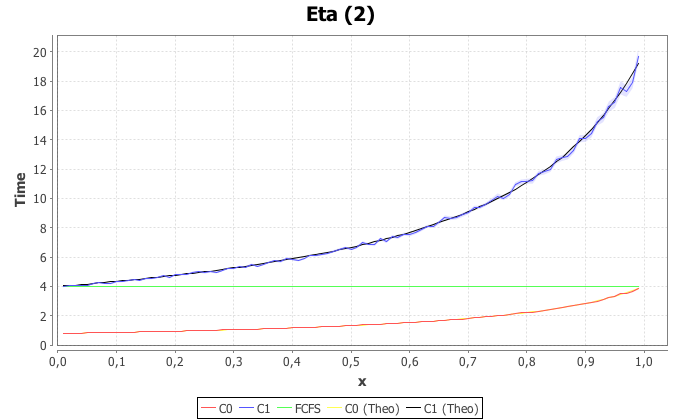
\includegraphics[width=\textwidth]{figures/MG1PRIO[2,mu1,r10000].png}
	\end{center}}
	\caption{Tempi medi di attesa medio nel sistema con coda a due classi di priorit\`a}
	\label{fig:mg1prio2}
\end{figure}

Analogamente a quando disposto nel caso della simulazione di sitema di tipo $M/G/1$, al termine dell'elaborazione verranno visualizzati i risultati grafici relativi alla simulazione svolta.

Nello specifico, la variabile $x$ viene fatta variare all'interno dell'intervallo (0,1), precedentemente suddiviso in $100$ quanti.

Gli andamenti degli $\overline{\eta}$ relativi alle varie classi mostrati all'interno dei grafici sono contraddistinti da una particolare notazione grafica che, attraverso l'utilizzo della medesima colorazione assegnata alla rispettiva classe, evidenzia gli intervalli di confidenza senza rendere difficoltosa l'interpretazione dei grafici, come invece accadrebbe con l'usuale notazione degli stessi.

Le diverse caratterizzazioni delle classi di priorit\`a, definite come da specifica richiesta, sono consultabili in tabella \ref{tab:mg1prioclasses}.


\begin{figure}[!h]{
	\begin{center}
	   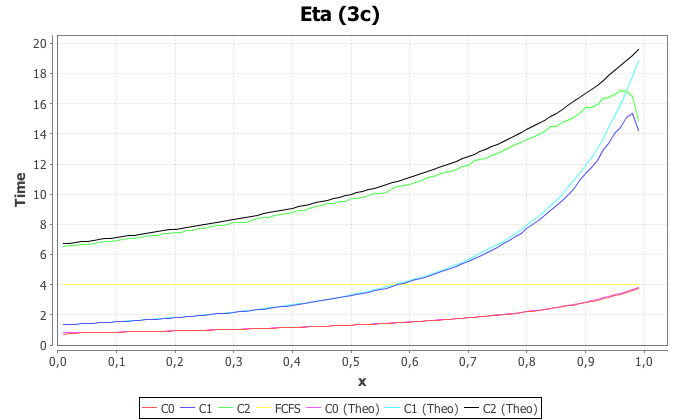
\includegraphics[width=\textwidth]{figures/MG1PRIO3c[mu=2,runs=10000,arrivals=1000].png}
	\end{center}}
	\caption{Tempi medi di attesa nel sistema con coda a tre classi (tipo c)}
	\label{fig:mg1prio3c}
\end{figure}


\begin{figure}[!h]{
	\begin{center}
	   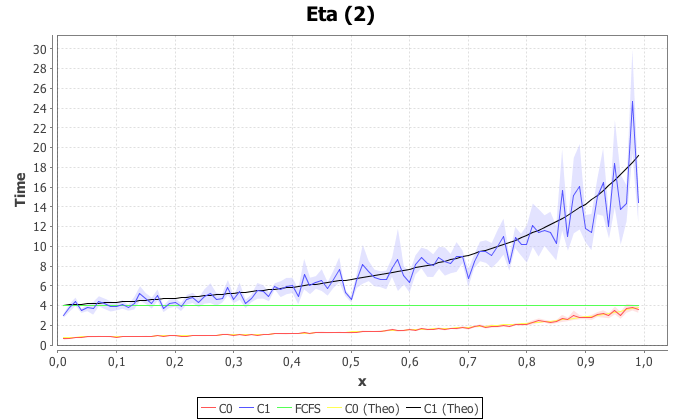
\includegraphics[width=\textwidth]{figures/mg1prio2low.png}
	\end{center}}
	\caption{Tempi medi di attesa nel sistema con coda a due classi (basso \#runs)}
	\label{fig:mg1prio2low}
\end{figure}

\subsubsection{Nota}

Nei grafici mostrati in figura \ref{fig:mg1prio2} e \ref{fig:mg1prio3c} non \`e possibile apprezzare a pieno gli intervalli di confidenza a causa della specificit\`a dei test eseguiti. In particolare le simulazioni relative alle suddette figure sono state compiute con quantit\`a di dati parcolarmente elevate, che  hanno determinato un'apprezzabile precisione dei risultati oltre ad una notevole durata in termini di tempo di simulazione. \\ Dualmente, la figura \ref{fig:mg1prio2low} \`e il risultato di una simulazione a due classi di priorit\`a effettuato specificando un numero molto inferiore di \emph{runs} e \emph{arrivi}, in maniera tale da mostrare l'incertezza dovuta alla discordanza tra i risultati: in particolare nell'immagine \`e possibile notare, che contorna ciascuna delle due linee, un'ombratura particolare che meglio identifica l'intervallo di confidenza puntuale associato al valor medio di $\eta$ al variare di $x$. 

\subsection{Analisi tecnica}

Anche in questo caso per l'implementazione della simulazione sono state seguite le linee guida presenti nella documentazione del corso. Il corpo della simulazione, definito all'interno della classe {\tt SimulatorRunners} (si veda fig \ref{fig:simulatorclass}), \`e suddiviso in una prima parte di parsing dell'input fornito dall'utente (metodo {\tt simulateMG1PrioWithVariableRhos(...)} durante il quale si definiscono i valori di $\rho_{1,2,(3)}$ e quindi dalla simulazione vera e propria, implementata all'interno del metodo {\tt simulateMG1Prio(...)}.

Tale metodo si appoggia sulla concretizzazione della classe astratta {\tt Simulator}, {\tt FCFSSimulator}, in cui si implementa un simulatore di tipo singolo servitore, con pi\`u code di attesa a decrescente grado di priorit\`a, ciascuna ordinata in base al semplice tempo di arrivo, {\tt OccurenceTime}. \\ Si vuole qu\`i inoltre notare che i singoli eventi che accadono all'interno del simulatore (arrivi e partenze) vengono mappati in analoghe classi ({\tt Event}, {\tt Arrival} e {\tt Departure} rispettivamente) organizzate in una gerarchia che vede sia gli arrivi che le partenze come specializzazioni del generico (e astratto) evento. Inoltre, come scelta progettuale, si \`e deciso di non includere nei singoli eventi anche la relativa politica di ordinamento, che viene invece specificata di volta in volta in classi appositamente create, derivanti da {\tt ComparableEvent}, le quali fungono da \emph{wrapper} dello specifico evento e ne stabiliscono i criteri di ordinamento; nel caso in questione una particolare sottoclasse di {\tt ComparableEvent}, {\tt OccurrenceTimeComparedEvent}, stabilisce, come politica, un ordinamento semplicemente basato sul tempo di occorrenza dell'evento: \emph{first-come-first-served}.










\chapter{Simulazioni opzionali}
\label{ch:optional}

\section{Stima della probabilit\`a di stato del sistema $M/G/1$}

Il calcolo ed il grafico relativi alla probabilit\`a di stato $k$ all'interno di un sistema a coda $M/G/1$ sono accedibili attraverso la scheda relativa al sistema $M/G/1$, le cui caratteristiche sono state precedentemente esposte (cap. \ref{ch:mg1}).

\begin{figure}[!h]{
	\begin{center}
	   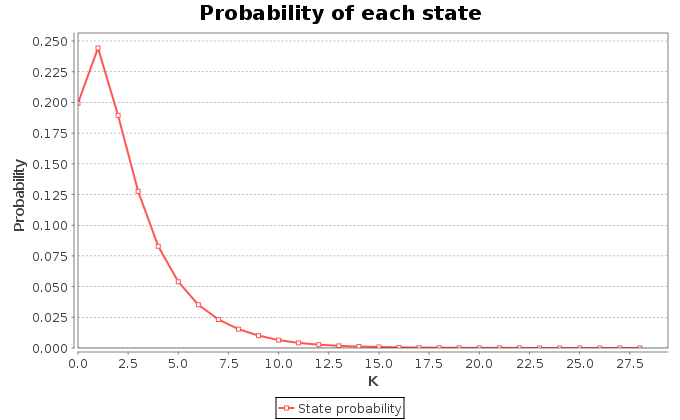
\includegraphics[width=\textwidth]{figures/mg1k.png}
	\end{center}}
	\caption{Probabilit`a di stato $k$, $\rho=0.8$, $\mu=1$, $N=100$, $arrivi=1000$ (Deterministic service time) }
	\label{fig:mg1k}
\end{figure}

All'utente viene lasciata la libert\`a di definire il grado di occupazione del servitore del sistema $\rho$, il tempo medio di servizio $\mu$, il numero di run da effettare $N$, il numero di arrivi per ciascuna run e, ovviamente, la tipologia di distribuzione. 

Come dati esemplificativi di questa gamma di simulazioni sono stati scelti quelli rappresentati in fig. \ref{fig:mg1k}, che descrive la probabilit\`a di stato di un sistema con tempo di servizio deterministico, e quelli di fig. \ref{fig:paretok}, raffigurante le probabilit\`a di stato di un sistema con tempo di servizio distribuito secondo Pareto.
\`E possibile notare come, a causa della maggior variabilit\`a dei tempi di servizio, il sistema con traffico di Pareto raggiunga stati di congestione caratterizzati da un alto numero di utenti nel sistema. Le probabilit\`a di stato infatti, sono non nulle anche con k pari a qualche centinaio di utenti.

\begin{figure}[!h]{
	\begin{center}
	   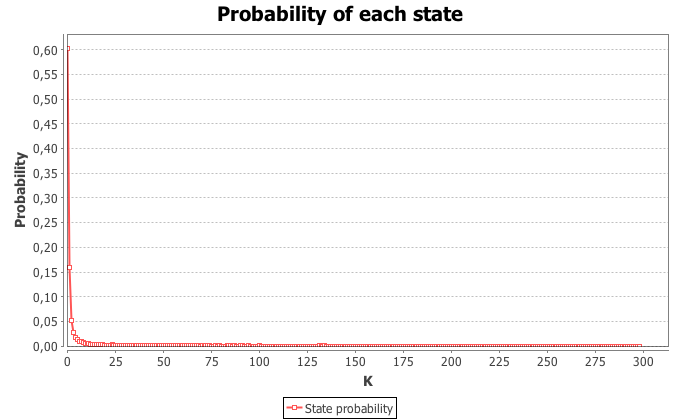
\includegraphics[width=\textwidth]{figures/statepareto.png}
	\end{center}}
	\caption{Probabilit`a di stato $k$, $\rho=0.5$, $\mu=2$, $N=100$, $arrivi=1000$ (Pareto service time) }
	\label{fig:paretok}
\end{figure}

\subsection{Analisi tecnica}

Analogamente a quanto visto in tutti casi precedenti ed in aderenza al modello definito per il simulatore, dopo un prima parte di handling da parte del pannello relativo all'interno dell'interfaccia grafica (classe {\tt MG1Panel}), si ricorre alla classe {\tt SimulationRunners}, ed in particolare al suo metodo:

$\cdot$ {\tt simulateMG1EvaluatingProbability(...)} \\
per l'esecuzione effettiva, mostrando il grafico di $P(k)$ in conclusione.

Tale metodo, per funzionare correttamente, si appoggia sul gi\`a precedentemente descritto {\tt FCFSSimulator}, utilizzato qu\`i con una sola classe di priorit\`a (quindi una singola coda di attesa), il quale fornisce un metodo ad-hoc, {\tt getStatesProbability}, che restituisce, per ogni stato $K(t)$ raggiunto durante la simulazione, la sua probabilit\`a empirica, calcolata semplicemente tenendo traccia del tempo totale trascorso in quel particolare stato, diviso per il tempo totale della simulazione.

\newpage
\section{Sistema $M/G/1$ con politica \emph{ Shortest Job Next}}

Come seconda simulazione opzionale si \`e scelto di implementare un sistema a coda con politica di tipo {\em shortest job first}. 

In questo caso all'utente viene chiesto di determinare, oltre agli usuali parametri di simulazione, il numero di step da considerare ed un moltiplicatore di $\theta$ al fine di eseguire la discretizzazione logaritmica dei tempi di servizio degli utenti del sistema in funzione della costruzione del grafico visualizzato al termine dell'elaborazione.

Il moltiplicatore di $\theta$, in particolare, andr\`a a determinare l'estensione del grafico lungo l'asse delle ascisse influendo dunque sulla porzione di curva visualizzata.

\begin{figure}[!h]{
	\begin{center}
	   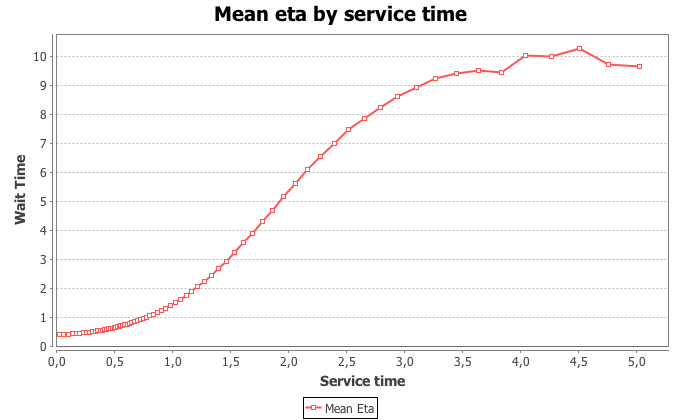
\includegraphics[width=\textwidth]{figures/MG1SJN[rho_08,mu_05,runs_1000,arrivals_100000,steps_30,mult_10].png}
	\end{center}}
	\caption{$\overline\eta$ in funzione del tempo di servizio $\theta$}
	\label{fig:mg1sjn}
\end{figure}

In figura \ref{fig:mg1sjn} \`e possibile osservare l'esito di una simulazione con parametri: $\rho=0.8$, $\mu=0.5$, $N=1000$, arrivi$=100'000$, $0\rightarrow\theta$ steps$=30$ ed intervallo di considerazione pari a $10\theta$: si noti come attraverso la discretizzazione logaritmica gli intervalli siano pi\`u concentrati e di dimensioni pi\`u ridotte intorno alla media (2) e di dimensioni maggiori man mano che ci si allontana dalla stessa.

\subsection{Note sulla discretizzazione logaritmica}
Al fine di ottenere simulazioni pi\`u accurate, l'intervallo continuo $\theta$ viene discretizzato, anzich\`e mediante una classica funzione lineare, ricorrendo ad una pi\`u complessa funzione logaritmica in modo tale da avere una maggiore concentrazione di piccoli intervalli nell'intorno della media di $\theta$  stesso, dove \`e pi\`u probabile ottenere valori, e pochi intervalli sempre pi\`u grandi mano a mano che ci si allontana da $\overline{\theta}$. La funzione utilizzata risulta essere la seguente: \\

$f(x) =	\left\{ \begin{array}{rcl}  
	-\log(-x+\overline{\theta}+b) + a + \overline{\theta} & \mbox{for} & x<\theta \\ 
	\log(+x-\overline{\theta}+b) - a + \overline{\theta} & \mbox{for} & x\leq\theta \\ 
	a = \overline{\theta}\cdot \frac{10^{-\overline{\theta}}}{1 - 10^{-\overline{\theta}}} & & \\ 
	b = log(a) \end{array} 
 \right.$ 	\\

parametrizzata rispetto a $\overline{\theta}$, $a$ e $b$; dove 
\begin{itemize}
\item $\overline{\theta}$ \`e la media attorno alla quale i valori di $\theta$ si dispongono
\item i parametri $a$ e $b$ dipendono da $\overline{\theta}$ e servono per forzare la funzione $f(x)$ a passare dai punti $(0,0)$ e $(\overline{\theta},\overline{\theta})$
\end{itemize}

Utilizzando una scala lineare lungo l'asse delle $y$, con passo costante e arbitrariamente definibile, e calcolandosi i relativi valori di $x$ mediante $f^{-1}(y)$ si ottengono i suddetti intervalli concentrati attorno al valore di $\overline{\theta}$; il valore scelto come rappresentativo di ciascun intervallo \`e semplicemente il valore mediano $x_{c} = \frac{x_{i} + x_{i + 1}}{2}$ \\

\begin{figure}[!h]{
	\begin{center}
	   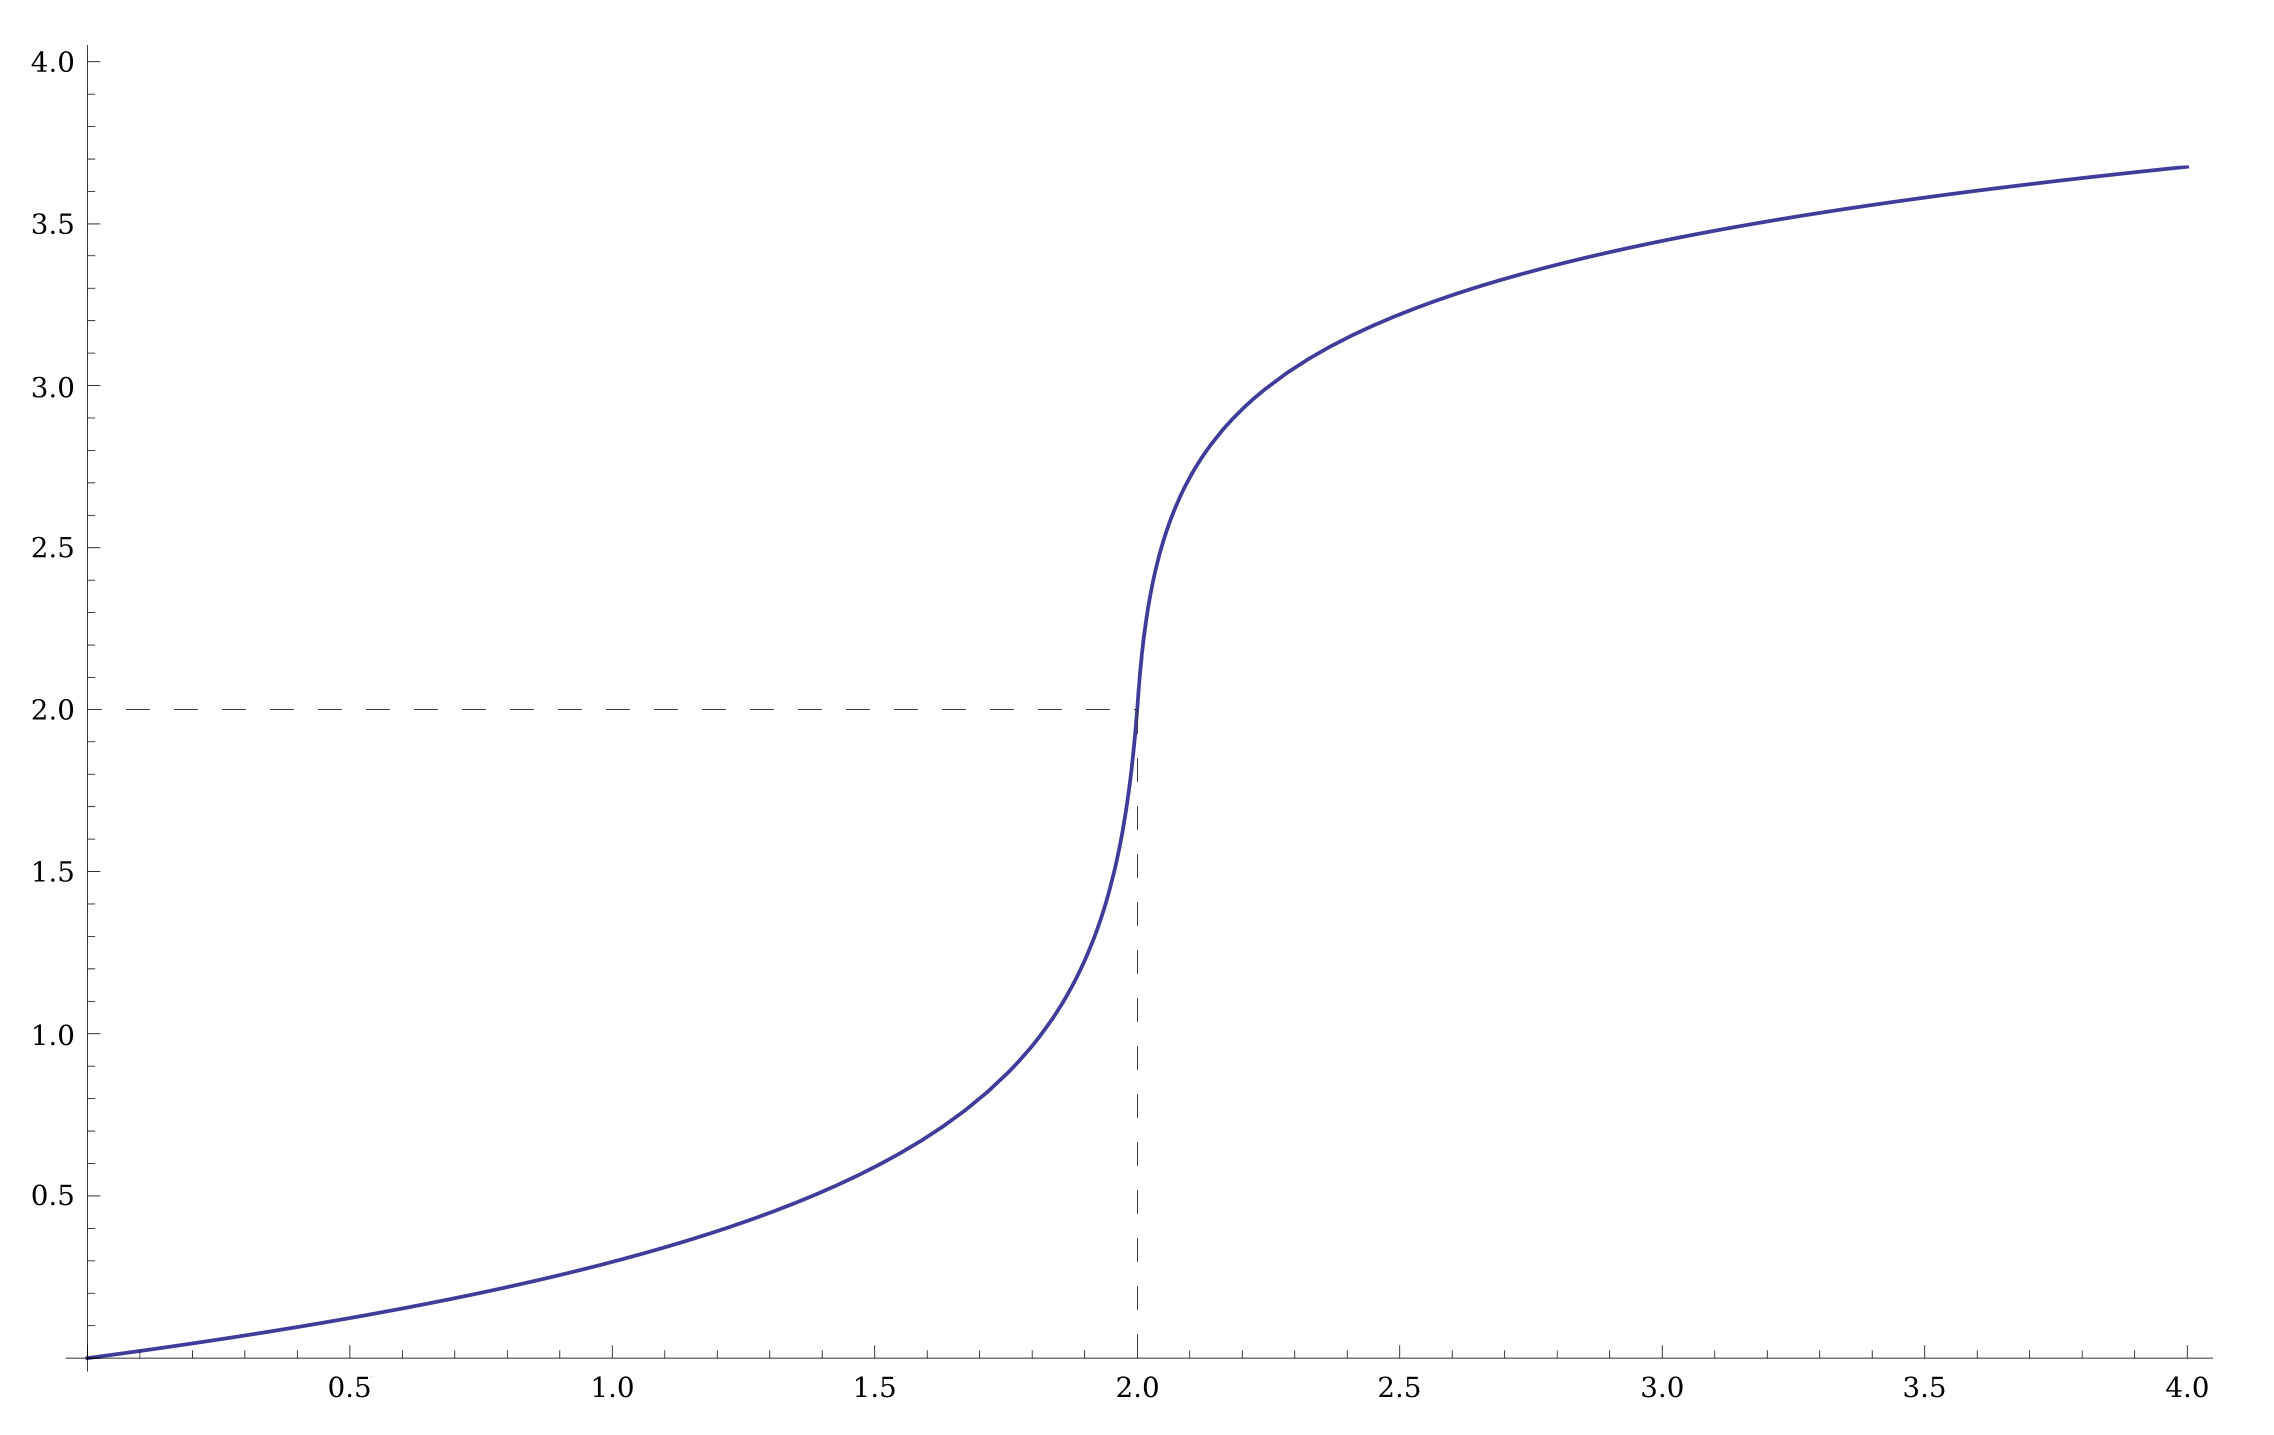
\includegraphics[width=\textwidth]{figures/loga-ritmo-per-ballare.png}
	\end{center}}
	\caption{esempio di una funzione logaritmica usata per la discretizzazione nel caso di $\overline{\theta} = 2$}
	\label{fig:log}
\end{figure}

\subsection{Analisi tecnica}

Nei casi precedenti, l'utilizzo (indiretto) della classe astratta {\tt Simulator} era sempre avvenuto attraverso la sua specializzazione {\tt FCFSSimulator}, sulla quale \`e stata implementata una gestiene di tipo FIFO.

Per la diversa tipologia di politica si \`e quindi provveduto all'implementazione della classe {\tt SJNSimulator}, che unitamente al metodo {\tt simulateMG1SJN(...)} della classe {\tt SimulationRunners} permette la definizione della nuova dinamica all'interno del sistema.

La classe {\tt SJNSimulator} concretizza la classe astratta {\tt Simulator} e, analogamente alla classe {\tt FCFSSimulator}, utilizza un'apposita specializzazione di {\tt ComparableEvent}, {\tt ServiceTimeComparedEvent}, la quale adotta come criterio di ordinamento il {\tt ServiceTime} di ciascun evento: eventi pi\'u corti verranno serviti prima. Una differenza importante rispetto al FCFSSimulator risiede nel calcolo dell'$\overline{\eta}$ per ciascuna \emph{classe}: infatti in questo caso, la coda di attesa \`e unica, non esistono priorit\`a differenti, ma viene richiesto di tenere traccia dei differenti tempi di attesa in base ad una discretizzazione dell'intervallo del tempo di servizio, $\theta$. A questo fine, ad ogni tempo di servizio, tramite la classe {\tt LogaritmicQuantizator}, viene assegnata una classe di appartenenza, con la quale aggiornare il relativo valore di attesa in coda.

\subsubsection{Nota finale}
Per ulteriori dettagli tecnici sull'implementazione del simulatore si rimanda alla consultazione della documentazione specifica (javadoc) contestualmente prodotta.

\chapter{Struttura del codice sorgente}
\label{ch:optional}

\section{Struttura dei package}

Il codice sorgente \`e stato strutturato in tre package principali al fine di ottenere una buona separazione delle varie componenti presenti all'interno del progetto.

Si riporta di seguito la struttura completa dei package:

{\tt
\begin{itemize}
\item[\textbullet] gui
	\begin{itemize}
		\item[\textbullet] panels
	\end{itemize}
\item[\textbullet] simulator
	\begin{itemize}
		\item[\textbullet] distribution
		\item[\textbullet] events
		\item[\textbullet] misc
		\item[\textbullet] random
	\end{itemize}
\item[\textbullet] launchers
\end{itemize}
}

All'interno del package {\tt gui} sono state implementate le classe dedicate all'interfaccia grafica. Il package {\tt gui.panels} contiene i pannelli dell'interfaccia dedicati a ciascuna tipologia di simulazioni.

Il package {\tt simulator} contiene la gerarchia di classi relative all'implementazione dei vari meccanismi di simulazione, fattorizzando le operazioni comuni all'interno della classe padre {\tt Simulator}.
\`E stato necessario implementare numerose tipologie di simulatore poich\'e in ciascuna delle politiche di scheduling considerate gli eventi da elaborare vengono gestiti in maniera specifica.
I package {\tt distribution}, {\tt events}, {\tt misc} e {\tt random}, contenuti all'interno di {\tt simulator}, contengono le classi utilizzate dal simulatore per modellare eventi, distribuzioni di numeri casuali e le implementazioni dei metodi utili ai fini dei calcoli statistici.

Il package {\tt launcher} contiene gli entry-point dell'applicazione: in particolare la classe {\tt SimulatorGUI} provvede all'avvio del simulatore, mentre gli ulteriori metodi presenti al suo interno avviano alcune interessanti simulazioni accessorie non accedibili dall'interfaccia grafica principale.

\chapter{Conclusioni}

\section{Simulatore di teletraffico}

L'utilizzo di un simulatore di teletraffico ha dato la possibilit\`a di andare a valutare il comportamento di sistemi di servizio noti a fronte di richieste inoltrate da popolazioni generate artificialmente ma caratterizzate da comportamenti riconducibili a casi reali. L'aderenza tra i modelli di traffico generati ed i corrispettivi teorici \`e garantita dalle specifiche dei generatori di numeri pseudo-casuali ai quali si \`e fatto ricorso.
\\

In termini generali \`e comunque bene tenere conto del fatto che la simulazione di teletraffico rappresenti in s\'e un problema di grande complessit\`a. Al di l\`a delle considerazioni sulla qualit\`a dei numeri pseudo-casuali ai quali si fa riferimento \`e infatti importante tenere conto della realt\`a dei sistemi che si intendono simulare, nei quali le dinamiche di funzionamento sono determinate da grandi quantit\`a di variabili, spesso difficili anche da identificare, oltre che da esprimere attraverso un modello. 
\\

Fatta questa precisazione, la creazione e l'utilizzo di un simulatore possono sicuramente rappresentare una risorsa di indiscutibile utilit\`a per la sintesi ed il dimensionamento di sistemi di teletraffico per applicazioni reali, rendendo possibile un'immediata rappresentazione e valutazione di caratteristiche e dinamiche altrimenti difficili da contemplare.


%%%%%%%%%%%%%%%%%%%%%%%%%
% Ending part of the	%
%	document	%
%%%%%%%%%%%%%%%%%%%%%%%%%
\backmatter

%\input{./appendix/appendix.tex}

%bibliography
\begin{thebibliography}{20}

\bibitem{callegati01}
  F. Callegati, G. Corazza
  \emph{``Elementi di teoria del traffico per le reti di telecomunicazioni''}
  Societ\`a Editrice Esculapio, Bologna
  2006

\bibitem{cerroni01}
  W. Cerroni
  \emph{Lucidi del secondo modulo del corso di Progetto di reti di telecomunicazioni}
  DEIS, Bologna
  2010

\bibitem{matsumoto}
  M. Matsumoto, T. Nishimura
  \emph{``Mersenne Twister: A 632-dimensionally equidistribuited uniform pseudorandom number generator''}
  Keio University
  1997

\bibitem{jfreechart}
  David Gilbert
  \emph{``The JFreeChart Class Library - Developer Guide (v.1.0.9)''}
  Object Refinery Limited
  2000-2008


\end{thebibliography}



% list of the figures
\listoffigures


% list of the tables
\listoftables


% document end
\end{document}
